\documentclass[10pt]{article}
\usepackage[margin=1in]{geometry}
\usepackage{amsmath,amssymb}
\usepackage{graphicx}
\usepackage{booktabs}
\usepackage{hyperref}
\usepackage{xcolor}
\usepackage{amsthm}
\graphicspath{{figures/}}
\newtheorem{proposition}{Proposition}

\title{GIR-Field: Gauge-Identifiable Exposure Field Learning for Uneven Low-Light Enhancement}
\author{Draft generated from formal frozen-evidence protocol}
\date{2026-07-06}

\begin{document}
\maketitle

\begin{abstract}
Low-light enhancement is usually judged by RGB fidelity, yet a model can improve PSNR while learning an exposure field with the wrong spatial structure. This paper studies that failure mode through \emph{gauge-identifiable exposure-field learning}. We show that local exposure fields are ambiguous up to an additive image-level gauge, and decompose them into a gauge-free spatial shape $S$ and an absolute gauge $\mu$. Based on this decomposition, we introduce centered exposure-shape calibration and UEFB-G, a gauge-controlled evaluation protocol that separates RGB fidelity, global gauge error, and local exposure-shape error. In a full frozen-evidence audit over 500 UEFB-v2 images, 100 LOL-v2-real images, and 100 LOL-v2-synthetic images, centered E-shape calibration improves UEFB gauge-free shape correlation over joint training by +0.1581 (95\% CI [0.1369, 0.1791], FDR $q=2.18\times10^{-43}$), while also improving real and synthetic PSNR by +0.6963 dB and +0.6321 dB. We further show a PSNR-only misranking: an A-gate variant obtains higher UEFB PSNR but negative exposure-shape correlation, whereas the centered E-shape model yields physically coherent fields. The resulting contribution is not a SOTA restoration claim; Retinexformer remains stronger in RGB fidelity. Instead, GIR-Field reframes uneven low-light enhancement as a problem of gauge-identifiable field learning, benchmark design, and claim-calibrated failure analysis.
\end{abstract}

\section{Introduction}
\label{sec:introduction}

Low-light enhancement has made steady progress by improving RGB reconstruction quality. Retinex-inspired decompositions, zero-reference curve estimation, and transformer-based restoration models have all improved the visual and numerical fidelity of enhanced images~\cite{land1971retinex,wei2018deepretinex,zhang2019kind,guo2020zerodce,li2021zerodcepp,cai2023retinexformer}. Yet the experiments in this work begin from an inconvenient observation: image fidelity can improve while the model's local exposure field becomes physically less meaningful. On UEFB-v2, an A-gate variant reaches a higher PSNR than our centered E-shape model, but its gauge-free exposure-shape correlation is negative. A PSNR-only benchmark would therefore select a model whose exposure field points in the wrong spatial direction.

This observation matters because exposure-field models are usually motivated not only as black-box enhancers, but also as interpretable mechanisms for uneven illumination. If the field is not identifiable, then the method's physical story becomes fragile: a model may look better in RGB space while failing the very exposure interpretation it claims to provide. The central question of this paper is therefore not whether another network can beat the strongest restoration baseline. Instead, we ask: \emph{what does it mean for a local exposure field to be identifiable, and how should we evaluate such a field when RGB fidelity and field consistency disagree?}

We argue that the core difficulty is gauge ambiguity. A local exposure field is naturally defined in log-luminance space, but gradient-domain or Poisson-like constraints are insensitive to additive shifts. Thus, the absolute gauge of the field and its spatial shape are entangled. This motivates the decomposition $E=S+\mu$, where $S=E-\mathrm{mean}(E)$ is a gauge-free spatial shape and $\mu$ is the image-level gauge. Under this view, a model should not be judged only by absolute field error or output PSNR; it should be evaluated by how well it predicts shape, gauge, and RGB output separately.

To operationalize this idea, we propose GIR-Field, a gauge-identifiable exposure-field learning and evaluation framework. The method uses centered exposure-shape calibration to supervise spatial exposure structure while ignoring additive gauge shifts. The evaluation protocol, UEFB-G, reports output-only metrics for all methods and internal-field metrics only for methods with explicit exposure predictions. It further includes gauge perturbations that test whether a metric can distinguish global gauge shifts from local shape distortions.

Our full frozen-evidence audit supports the need for this reframing. Across 500 UEFB-v2 test images, 100 LOL-v2-real images, and 100 LOL-v2-synthetic images, centered E-shape calibration improves UEFB gauge-free shape correlation over joint training by +0.1581 with a 95\% bootstrap confidence interval of [0.1369, 0.1791] and FDR-corrected $q=2.18\times10^{-43}$. It also improves real PSNR by +0.6963 dB and synthetic PSNR by +0.6321 dB. Conversely, the PSNR-high A-gate model has negative exposure-shape correlation on all internal-field splits, showing that PSNR-only ranking can hide a physically wrong field.

We deliberately calibrate the claim boundary. GIR-Field does not outperform Retinexformer~\cite{cai2023retinexformer} in RGB fidelity, and we do not present it as a SOTA low-light restoration method. Retinexformer remains substantially stronger on LOL-v2-real and LOL-v2-synthetic. The contribution is instead methodological: we identify a gauge ambiguity in exposure-field learning, provide metrics and perturbations that separate gauge and shape errors, and show that a centered shape objective can produce statistically reliable field improvements without sacrificing paired fidelity.

Our contributions are:
\begin{itemize}
    \item We formalize local exposure-field learning as a gauge-identifiability problem, decomposing $E$ into a gauge-free spatial shape $S$ and image-level gauge $\mu$.
    \item We introduce centered exposure-shape calibration, a gauge-invariant objective that improves exposure-shape correlation and paired fidelity in a full local audit.
    \item We propose UEFB-G, a gauge-controlled evaluation protocol that separates output-only metrics from internal-field metrics and uses perturbations to distinguish global gauge shifts from local shape distortions.
    \item We provide a claim-calibrated failure audit: PSNR-only ranking can select a physically incoherent exposure field, and recoverability risk is predictable but not yet well calibrated.
\end{itemize}

\section{Related Work}
\label{sec:related_work}

\subsection{Low-light image enhancement}

Low-light image enhancement has been studied through both physical image formation models and data-driven restoration networks. Retinex theory models an image as the interaction of reflectance and illumination~\cite{land1971retinex}, motivating decomposition-based methods that estimate and manipulate illumination maps. RetinexNet~\cite{wei2018deepretinex} and KinD~\cite{zhang2019kind} extend this idea with neural decompositions and enhancement modules, while Zero-DCE~\cite{guo2020zerodce} and Zero-DCE++~\cite{li2021zerodcepp} formulate enhancement as curve estimation without paired supervision. More recent transformer-based methods, including Retinexformer~\cite{cai2023retinexformer}, substantially improve RGB restoration fidelity. A 2024--2026 refresh shows that the field is also moving toward state-space and exposure-correction architectures~\cite{weng2024mamballie,dong2024ecmamba,li2024osmamba}, unfolding and Retinex-consistency designs~\cite{he2025unfoldir,xu2025consistretinex}, and diffusion or flow-based restoration~\cite{xu2025boostingfidelityfo,wei2025illumflow}. These methods establish strong enhancement baselines, and our experiments confirm that Retinexformer remains far ahead of our RLEF variants on LOL-v2 synthetic PSNR.

Our work is not positioned as a stronger restoration network. Instead, it studies a failure mode that standard restoration metrics can hide: a method may improve RGB fidelity while learning an exposure field whose spatial structure is physically inconsistent. This shifts the question from ``which enhancer has the highest PSNR?'' to ``when an enhancer claims to learn an exposure field, is that field identifiable and correctly evaluated?''

\subsection{Exposure fields and physical interpretability}

Many physically motivated enhancement methods use illumination maps, exposure maps, transmission-like fields, or Retinex factors as interpretable internal variables. Such variables are attractive because they promise more than black-box restoration: they suggest that the model has discovered a meaningful correction structure. Recent work has also made non-uniform exposure explicit, including dual uniform/non-uniform LLIE~\cite{perez-zarate2024alen}, spatially non-uniform exposure correction~\cite{li2026rethinkingexposure}, log-domain intensity--chromaticity decoupling~\cite{bai2026rethinkinglowlight}, and illumination-field or Gaussian light-field modeling~\cite{chen2026aigsnet,chen2026gaussianlightfield}. These trends make identifiability more important, not less. In gradient-domain or Poisson-like objectives, adding a constant to an exposure field preserves local gradients, so absolute gauge and spatial shape can be confounded. A field may therefore appear plausible under one metric while being wrong under another.

GIR-Field addresses this issue by separating the field into a gauge-free shape $S$ and an image-level gauge $\mu$. This is a modest but important shift: rather than treating exposure error as a single scalar, we ask whether an error comes from global gauge shift, local shape distortion, or output restoration failure. This decomposition is the basis for both our training objective and our evaluation protocol.

\subsection{Benchmarks and metric design for enhancement}

Paired datasets such as LOL-v2 and low-light raw-image benchmarks~\cite{chen2018sid} support full-reference evaluation with PSNR and SSIM, while unpaired real collections are often evaluated with no-reference metrics or visual inspection. Recent challenge and evaluation work reinforces that LLIE assessment is becoming broader but remains mostly output-centered: NTIRE 2025/2026 challenge reports emphasize restoration efficiency and quality~\cite{liu2025ntire2025challenge,yan2026ntire2026challenge}, multi-intensity evaluation probes robustness across illumination levels~\cite{pilligua2025evaluatinglowlight}, and low-light quality assessment studies artifacts such as noise, color shift, structural damage, and over-exposure~\cite{sun2026leiqassessor}. These metrics are useful but incomplete for exposure-field models. PSNR can reward a model that reconstructs RGB values well while giving no guarantee that the internal exposure map is physically meaningful. No-reference scores can provide additional evidence, but they are not stable enough to support a main superiority claim.

UEFB-G is designed for this gap. It does not replace PSNR; instead, it prevents PSNR from being the only ranking signal. Output-only metrics remain available for any method, including Retinexformer, Zero-DCE++, and KinD++. Internal-field metrics are reported only when a method explicitly predicts an exposure field. This distinction avoids unfairly penalizing black-box baselines for not exposing internal variables while still testing the physical claims of exposure-field methods.

\subsection{Calibration, selective prediction, and recoverability risk}

The recoverability question is related to selective prediction and calibration: an enhancer should know where enhancement is beneficial, harmful, or uncertain. Prior work in calibrated prediction emphasizes not only the accuracy of a score but also whether the score's confidence matches empirical risk. In our setting, DGB-style routing experiments suggested that route usage alone is not sufficient: sending more samples through a restoration or safe path does not guarantee better output quality.

We therefore treat recoverability as a diagnostic audit rather than a solved module. Our lightweight risk probe reaches AUC around 0.766, showing that harmful enhancement is predictable from image and field statistics, but ECE around 0.281 shows that calibration remains weak. This result supports future work on recoverability-aware enhancement, but it does not justify a main method claim.

\subsection{Positioning of this work}

Compared with restoration-centered LLIE methods, GIR-Field contributes a claim-calibrated evaluation and mechanism analysis. Compared with Retinex-style decomposition, it focuses on the gauge ambiguity of the exposure field and explicitly separates global gauge from spatial shape. Compared with benchmark-only work, it provides a concrete mechanism---centered E-shape calibration---that improves gauge-free shape correlation and paired fidelity in a formal frozen-evidence audit. The resulting paper is therefore best read as a mechanism-and-benchmark contribution rather than a SOTA restoration paper.

\section{Method}
\label{sec:method}

\subsection{Motivation: when image fidelity misleads exposure-field learning}

Low-light image enhancement is commonly evaluated by image-fidelity metrics such as PSNR and SSIM. These metrics are necessary, but they do not determine whether an exposure-field model has learned a physically meaningful local exposure structure. Our formal audit exposes this gap directly: on UEFB-v2, the M4 A-gate variant obtains the highest UEFB PSNR among internal mechanisms (18.6530), yet its gauge-free exposure-shape correlation is negative ($S_{corr}=-0.1393$). In contrast, M4J\_ES has a slightly lower UEFB PSNR (17.9811) but a strongly positive exposure-shape correlation ($S_{corr}=0.4399$). Thus, PSNR-only evaluation can select a model whose RGB output is locally plausible while its exposure field points in the wrong spatial direction.

We therefore formulate the task not as another SOTA low-light restoration model, but as \emph{gauge-identifiable exposure-field learning}: a model should separate gauge-free exposure shape from absolute image-level gauge, and the benchmark should report when image fidelity and exposure-field identifiability disagree.

\subsection{Gauge ambiguity of local exposure fields}

Let $I_l$ denote a low-light image and $I_h$ the paired normally exposed target. Let $Y_l$ and $Y_h$ be their luminance channels. A diagnostic target exposure field can be written as
\begin{equation}
E^*(x) = \log(Y_h(x)+\epsilon) - \log(Y_l(x)+\epsilon),
\end{equation}
where $x \in \Omega$ indexes spatial position and $\epsilon$ is a small constant. In gradient-domain or Poisson-like formulations, the field $E$ is ambiguous up to an additive constant: $E$ and $E+c$ have the same local gradient structure. A model that optimizes an absolute field loss can therefore entangle global gauge error with spatial shape error, while a model that optimizes only RGB reconstruction can obtain high PSNR with an incorrect exposure shape.

We decompose the exposure field into an image-level gauge and a zero-mean spatial shape:
\begin{equation}
\mu(E) = \frac{1}{|\Omega|}\sum_{x\in\Omega} E(x), \qquad
S(E)(x) = E(x) - \mu(E),
\end{equation}
so that
\begin{equation}
E(x) = S(x) + \mu, \qquad \sum_{x\in\Omega} S(x)=0.
\end{equation}
Under the zero-mean constraint, the decomposition is unique: $S$ represents gauge-free exposure shape, while $\mu$ represents absolute exposure gauge. This turns the equivalence class $E \sim E+c$ into two separately measurable components.

\begin{proposition}[Gauge-identifiable shape/gauge decomposition]
For any exposure field $E:\Omega\rightarrow\mathbb{R}$ on a finite image domain, the pair $(S,\mu)$ defined by $\mu=|\Omega|^{-1}\sum_{x\in\Omega}E(x)$ and $S=E-\mu$ is the unique decomposition satisfying $E=S+\mu$ and $\sum_{x\in\Omega}S(x)=0$. Moreover, for any additive gauge shift $E'=E+c$, the shape is invariant, $S(E')=S(E)$, while the gauge shifts by $c$, $\mu(E')=\mu(E)+c$.
\end{proposition}
\begin{proof}
Existence follows directly from the definitions. If $E=S_1+\mu_1=S_2+\mu_2$ and both $S_1,S_2$ have zero spatial mean, then taking spatial means gives $\mu_1=\mu_2=\mathrm{mean}(E)$, hence $S_1=S_2=E-\mathrm{mean}(E)$. For $E'=E+c$, centering cancels the constant shift, so $S(E')=E+c-\mathrm{mean}(E+c)=E-\mathrm{mean}(E)=S(E)$, while $\mu(E')=\mu(E)+c$.
\end{proof}

This proposition justifies reporting shape and gauge separately. A metric that only reports absolute field error cannot tell whether an error comes from $S$ or $\mu$; UEFB-G reports both.

\subsection{Centered exposure-shape calibration}

To make exposure-field supervision invariant to additive gauge shifts, we use a centered low-pass exposure-shape loss. Let $\mathcal{L}_{LP}$ be an average low-pass filter and $C(A)=A-\mathrm{mean}(A)$ be spatial centering. The shape loss is
\begin{align}
\mathcal{L}_{shape} &= 1 - \mathrm{corr}\left(C(\mathcal{L}_{LP}(\hat{E})), C(\mathcal{L}_{LP}(E^*))\right) \\
&\quad + \beta \|\nabla \hat{E} - \nabla E^*\|_1 .
\end{align}
The first term ignores global gauge shifts and compares low-frequency exposure shape; the second term preserves local spatial structure. In our implementation the low-pass kernel size is 7 and $\beta=0.1$; the default P3c setting uses $e\_shape=0.05$.

\subsection{UEFB-G: gauge-controlled evaluation}

We distinguish two kinds of metrics. Output-only metrics can be applied to any enhancement method, including black-box baselines: PSNR, SSIM, local exposure error, over/under exposure ratio, and identity drop. Internal-field metrics apply only to methods that explicitly predict an exposure field:
\begin{align}
\mathrm{S\_MAE} &= \|S(\hat{E}) - S(E^*)\|_1, \\
\mathrm{Gauge\_MAE} &= |\mu(\hat{E}) - \mu(E^*)|, \\
\mathrm{S\_corr} &= \mathrm{corr}(S(\hat{E}), S(E^*)).
\end{align}
Black-box methods such as Retinexformer, Zero-DCE++, and KinD++ are therefore compared only on output metrics; their internal-field metrics are marked N/A rather than imputed.

To verify that these metrics separate error types, we construct gauge perturbations on UEFB-G targets: global shifts $E'=E+c$, zero-mean local distortions $E'=E+\delta(x)$ with $\mathrm{mean}(\delta)=0$, and mixed distortions $E'=E+c+\delta(x)$. A correct gauge-controlled metric should ignore the first perturbation for shape evaluation but penalize the second.

\subsection{Recoverability risk as a diagnostic probe}

Finally, we audit recoverability without reviving the DGB router. For each local patch, we define a harmful-enhancement label by comparing the local MSE of the enhanced output to the input. A patch is harmful if enhancement increases local error relative to the low input. We train a lightweight logistic probe using low-image statistics, predicted output statistics, gate/recoverability proxies, exposure magnitude, and saturation proxy. This probe is not a method module; it measures whether recoverability risk is predictable and calibrated. In the formal run, the probe reaches AUC around 0.766 but ECE around 0.281, so we treat recoverability as a diagnostic signal rather than a solved contribution.

\section{Experiments}
\label{sec:experiments}

\subsection{Protocol}

We evaluate the proposed gauge-identifiability analysis under a formal frozen-evidence protocol. No new backbone training is performed, no DGB/P2F route is revived, and all internal methods use existing checkpoints. The full local evaluation includes 500 UEFB-v2 test images, 100 LOL-v2-real test images, and 100 LOL-v2-synthetic test images. With 9 internal variants, this produces 6300 per-image records. We use 5000 bootstrap samples for confidence intervals, paired Wilcoxon signed-rank tests~\cite{wilcoxon1945ranking} for paired comparisons, and Benjamini--Hochberg correction~\cite{benjamini1995fdr} for false-discovery-rate control.

The internal variants are M4, M4J, M4J\_ES, three P3c $e\_shape=0.05$ seeds, and three P3d $e\_shape=0.10$ seeds. External black-box baselines are Retinexformer~\cite{cai2023retinexformer}, Zero-DCE++~\cite{li2021zerodcepp}, and KinD++~\cite{zhang2019kind}. For black-box methods, internal exposure-field metrics are reported as N/A.

\subsection{Main results}

\begin{table*}[t]
\centering
\small
\begin{tabular}{lrrrrrr}
\hline
Method & UEFB PSNR & UEFB $S_{corr}$ & Real PSNR & Real $S_{corr}$ & Syn. PSNR & Syn. $S_{corr}$ \\
\hline
M4 A-gate & 18.6530 & -0.1393 & 17.4113 & -0.3314 & 13.9632 & -0.3372 \\
M4J joint & 18.0818 & 0.2818 & 19.5807 & 0.5007 & 16.5085 & 0.3690 \\
M4J\_ES & 17.9811 & 0.4399 & 20.2770 & 0.6483 & 17.1405 & 0.7992 \\
P3c $e=0.05$ (3 seeds) & 17.9145 & 0.4361 & 20.0206 & 0.7075 & 17.6783 & 0.8407 \\
P3d $e=0.10$ (3 seeds) & 18.1108 & 0.4491 & 19.8749 & 0.6856 & 17.6263 & 0.8347 \\
KinD++ & -- & N/A & 22.2109 & N/A & 19.2594 & N/A \\
Retinexformer & -- & N/A & 22.7939 & N/A & 25.6690 & N/A \\
Zero-DCE++ & -- & N/A & 18.4907 & N/A & 17.5764 & N/A \\
\hline
\end{tabular}
\caption{Formal full frozen-evidence results. Internal-field metrics are only reported for methods with explicit exposure-field predictions. Black-box baselines are output-only.}
\label{tab:main_results}
\end{table*}

Table~\ref{tab:main_results} shows that RGB fidelity and exposure-field identifiability can disagree. M4 obtains the strongest UEFB PSNR among the internal mechanisms but has negative $S_{corr}$ on all three internal-field splits. M4J\_ES and P3c reduce this contradiction: they do not outperform strong restoration baselines in fidelity, but they provide substantially more coherent exposure-shape predictions.

\subsection{Centered E-shape improves exposure-field identifiability}

\begin{table*}[t]
\centering
\small
\begin{tabular}{llccc}
\hline
Comparison & Metric & Delta & 95\% CI & FDR $q$ \\
\hline
M4J\_ES--M4J, UEFB & $S_{corr}$ & +0.1581 & [0.1369, 0.1791] & $2.18\times10^{-43}$ \\
M4J\_ES--M4J, Real & PSNR & +0.6963 & [0.4141, 0.9664] & $1.57\times10^{-5}$ \\
M4J\_ES--M4J, Synthetic & PSNR & +0.6321 & [0.4182, 0.8559] & $6.04\times10^{-8}$ \\
M4J\_ES--M4J, Synthetic & $S_{corr}$ & +0.4301 & [0.3499, 0.5160] & $1.72\times10^{-17}$ \\
\hline
\end{tabular}
\caption{Paired statistical tests for centered E-shape calibration. Positive deltas indicate improvement by M4J\_ES over M4J.}
\label{tab:eshape_stats}
\end{table*}

The central positive result is that M4J\_ES significantly improves gauge-free exposure-shape correlation over M4J. On UEFB-v2, the $S_{corr}$ improvement is +0.1581 with a 95\% bootstrap confidence interval of [0.1369, 0.1791] and FDR-corrected $q=2.18\times10^{-43}$. The same mechanism also improves real PSNR by +0.6963 dB and synthetic PSNR by +0.6321 dB. Thus, centered E-shape calibration is not merely an interpretability regularizer; in this setting it improves exposure-field identifiability while preserving or improving paired fidelity.

\subsection{PSNR-only ranking can select the wrong exposure field}

M4J\_ES has lower UEFB PSNR than M4 (17.9811 versus 18.6530), but it improves UEFB $S_{corr}$ by +0.5792 relative to M4, with 95\% CI [0.5361, 0.6230] and FDR-corrected $q=3.52\times10^{-64}$. This is the main empirical justification for UEFB-G: a PSNR-only benchmark would rank M4 above M4J\_ES, while a gauge-controlled benchmark reveals that M4 learns an exposure shape with the wrong sign.

\subsection{Gauge perturbation validates metric separation}

The gauge perturbation benchmark confirms that the proposed metrics separate global gauge error from local shape error. A global shift of +0.5 produces E\_MAE=0.5000 and Gauge\_MAE=0.5000, but S\_MAE=0.0000 and $S_{corr}=1.0000$. A local zero-mean shape distortion produces S\_MAE=0.2026 and $S_{corr}=0.6027$ while Gauge\_MAE remains 0.0000. The mixed perturbation combines both effects. This sanity check is important because it shows that UEFB-G is not simply adding more metrics; it operationalizes distinct failure modes.

\subsection{E-shape weight trade-off}

The three-seed comparison between P3c ($e\_shape=0.05$) and P3d ($e\_shape=0.10$) shows that a stronger shape weight is not automatically better. P3d slightly improves UEFB PSNR and $S_{corr}$, but P3c is more stable on real and synthetic splits: P3c has Real $S_{corr}=0.7075$ and Synthetic $S_{corr}=0.8407$, compared with 0.6856 and 0.8347 for P3d. We therefore keep P3c $e\_shape=0.05$ as the default and treat P3d as a stronger-shape control.

\subsection{External baselines and claim boundary}

Retinexformer remains substantially stronger in RGB fidelity: it obtains 22.7939 PSNR on LOL-v2-real and 25.6690 PSNR on LOL-v2-synthetic, compared with 20.0206 and 17.6783 for P3c. This gap prevents any SOTA restoration claim. The contribution of GIR-Field is instead a problem definition and evaluation framework for gauge-identifiable exposure-field learning.

\subsection{Recoverability risk is diagnostic, not solved}

The recoverability risk probe reaches AUC=0.7658 for M4J\_ES and AUC=0.7655 for P3c seed3407, suggesting that harmful local enhancement is predictable from image and field statistics. However, calibration remains weak: ECE is approximately 0.281 for both variants. We therefore use recoverability risk as diagnostic evidence and do not claim that a calibrated risk head solves enhancement.

\subsection{Summary of supported and unsupported claims}

The formal protocol supports three claims: (1) centered exposure-shape calibration improves gauge-free field identifiability; (2) UEFB-G exposes PSNR-only misranking; and (3) global gauge and local shape errors can be separated by the proposed metric decomposition. It does not support claims that DGB-RLEF is SOTA, that DGB resolves the tri-domain trade-off, that P3c/M4J\_ES outperforms Retinexformer, or that recoverability risk is solved.

\section{Diagnostic Figures and Captions}
\label{sec:figures}

\begin{figure}[t]
    \centering
    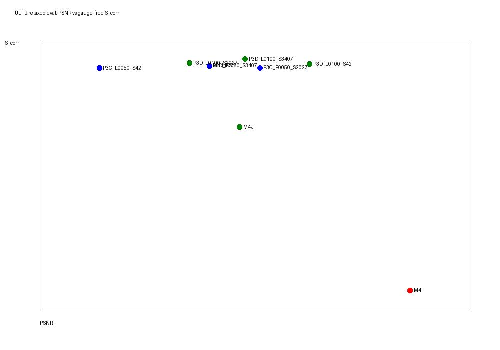
\includegraphics[width=0.95\linewidth]{fig_psnr_vs_scorr.pdf}
    \caption{\textbf{PSNR-only ranking can disagree with exposure-field identifiability.} The formal audit plots UEFB PSNR against gauge-free shape correlation $S_{corr}$ for internal variants. M4 obtains high UEFB PSNR but negative shape correlation, while M4J\_ES and P3c have lower or comparable PSNR with physically coherent positive $S_{corr}$. This is the central motivation for UEFB-G: a benchmark for exposure-field methods must report both output fidelity and field identifiability.}
    \label{fig:psnr_vs_scorr}
\end{figure}

\begin{figure}[t]
    \centering
    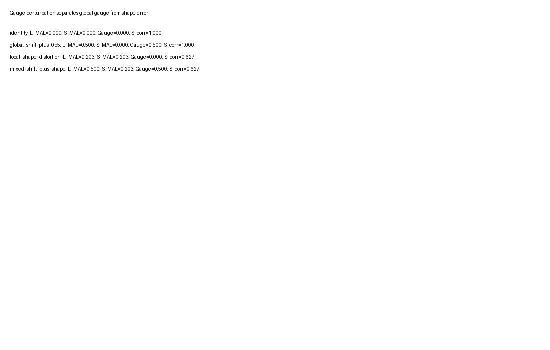
\includegraphics[width=0.95\linewidth]{fig_gauge_perturbation_bar.pdf}
    \caption{\textbf{Gauge perturbation separates global gauge shifts from local shape distortions.} A global shift $E'=E+0.5$ increases absolute E\_MAE and Gauge\_MAE but leaves S\_MAE at zero and $S_{corr}=1$, because the spatial shape is unchanged. A local zero-mean distortion changes S\_MAE and lowers $S_{corr}$ while leaving Gauge\_MAE near zero. This validates the metric decomposition used by UEFB-G.}
    \label{fig:gauge_perturbation}
\end{figure}

\begin{figure}[t]
    \centering
    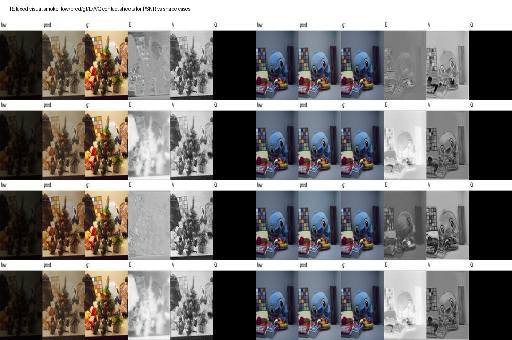
\includegraphics[width=0.95\linewidth]{fig_psnr_misranking_failure_grid.pdf}
    \caption{\textbf{Visual diagnostic grid for PSNR-vs-shape cases.} The grid shows low input, prediction, ground truth, and internal E/A/Q maps for representative UEFB cases. It is intended as a failure-analysis figure rather than a success-only qualitative panel: every row should be read with the question ``what does PSNR fail to reveal about the exposure field?''}
    \label{fig:failure_grid}
\end{figure}

\begin{figure}[t]
    \centering
    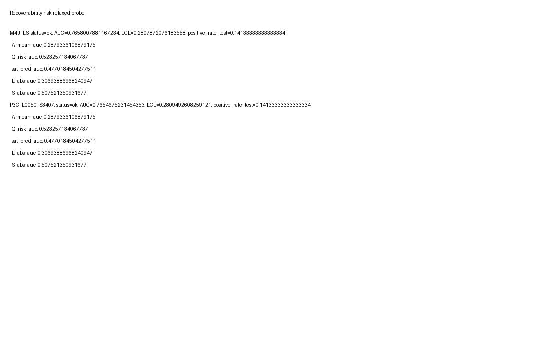
\includegraphics[width=0.95\linewidth]{fig_risk_reliability.pdf}
    \caption{\textbf{Recoverability risk has signal but remains calibration-limited.} The lightweight risk probe reaches AUC around 0.766, indicating that harmful local enhancement is predictable from image and field statistics. However, ECE remains around 0.281, so the probe is diagnostic rather than a calibrated decision module. This supports future recoverability-aware work but not a main claim that risk is solved.}
    \label{fig:risk_reliability}
\end{figure}

\section{Limitations}
\label{sec:limitations}

This work is claim-calibrated by design. First, GIR-Field is not a SOTA restoration method. Retinexformer remains substantially stronger in RGB fidelity on LOL-v2-real and LOL-v2-synthetic, so our claims are about exposure-field identifiability and evaluation rather than restoration dominance. Second, internal-field metrics apply only to methods that explicitly predict an exposure field. Black-box methods are evaluated fairly on output-only metrics, but they cannot be compared on $S_{corr}$ or Gauge\_MAE without adding an external field estimator. Third, the recoverability risk probe is not yet well calibrated: its AUC indicates signal, but its ECE remains too high for a deployed selective-enhancement module. Finally, the current formal audit uses local frozen checkpoints and local baselines; a submission-ready benchmark paper should further verify recent 2024--2026 low-light methods with official weights and protocols.

\section{Conclusion}
\label{sec:conclusion}

We presented GIR-Field, a gauge-identifiable view of local exposure-field learning for uneven low-light enhancement. The key finding is not that our model beats the strongest enhancer, but that standard image-fidelity metrics can select a physically incoherent exposure field. By decomposing $E$ into gauge-free shape $S$ and image-level gauge $\mu$, using centered E-shape calibration, and evaluating with UEFB-G, we separate RGB fidelity, global gauge error, and local shape error. A full frozen-evidence audit shows that centered E-shape significantly improves exposure-shape correlation over joint training while also improving real and synthetic PSNR. The resulting contribution is a mechanism and benchmark framework for claim-calibrated exposure-field research.

\appendix
\section{Negative-Route Audit}
\label{app:negative_routes}

The main paper deliberately does not hide failed routes. Table~\ref{tab:negative_route_audit} summarizes P5/P6/P7 and DGB-family runs that are retained as design rationale rather than promoted evidence. These runs are useful because they rule out tempting but insufficient explanations: teacher distillation, dataset-weighted reconstruction, scalar or identity gates, domain heads, real anchors, and DGB routing each move the tri-domain trade-off, but none provides a promoted joint model.

\section{Expanded Negative-Route Audit}
\label{app:negative_routes_expanded}

The stopped routes are not discarded implementation history; they are evidence about which explanations failed. The audit separates three failure modes. First, several routes improve one score by importing a new bias, such as a teacher output, domain weight, or real-anchor regularizer. Second, several routes improve an output metric while leaving exposure-field identifiability unresolved. Third, DGB-style routing changes path allocation but does not become a calibrated recoverability mechanism. Tables~\ref{tab:negative_route_family_summary} and~\ref{tab:negative_route_audit} preserve this evidence so that the paper does not overfit its story to the successful M4J\_ES/P3c route.

\paragraph{Distillation and domain weighting.} P5/P5B show why teacher distillation is not used as the main claim. The best P5 real score and the best P5 synthetic score occur under different temperature settings, and P5B introduces domain-specific weights while still not producing a promoted joint model. These runs support the decision to avoid a teacher-distillation contribution.

\paragraph{Structural and protection routes.} P6/P6B/P6C test whether capacity, synthetic reconstruction protection, or scalar gate protection can solve the tri-domain conflict. The answer is negative: synthetic protection increases synthetic scores at the cost of UEFB/real behavior, while gate protection remains a scalar control heuristic rather than a gauge-identifiable principle.

\paragraph{Domain heads and real anchors.} P7/P7B/P7C test whether domain adapters or real-anchor regularizers can stabilize real performance. They produce local improvements but remain domain-fragile. Since the paper claims gauge-identifiable exposure-field learning, not dataset-specific anchoring, these routes are kept as appendix evidence only.

\paragraph{DGB branch.} DGB and P2B--P2E routing variants are explicitly stopped. Their split-wise improvements are useful diagnostics, but every row in the consolidation table has promotion marked false. This is why the main paper does not revive DGB/P2F or present routing as solved recoverability.

\begin{table*}[t]
\centering
\scriptsize
\resizebox{\textwidth}{!}{%
\begin{tabular}{lrlrlrl}
\hline
Family & N & Best real variant & Real & Best synthetic variant & Synthetic & Audit conclusion \\
\hline
P5 distillation & 2 & P5\_RD\_T03 & 20.416 & P5\_RD\_T01 & 17.960 & Teacher distillation improves one split at a time and can depress synthetic fidelity; it is not a mechanism-level fix for gauge identifiability. \\
P5B domain distillation & 1 & P5B\_DW\_R03\_S005 & 19.366 & P5B\_DW\_R03\_S005 & 17.473 & Domain-weighted distillation uses domain-specific weighting and therefore weakens the clean mechanism claim while still failing to dominate all splits. \\
P6 structure & 1 & P6\_MS\_M4J\_ES & 20.197 & P6\_MS\_M4J\_ES & 17.598 & Structural backbone changes capacity and improves local behavior, but the gains are architecture-specific rather than an identifiable exposure-field principle. \\
P6B synthetic protection & 4 & P6B\_MS\_SYN105 & 19.996 & P6B\_MS\_SYN125 & 19.115 & Increasing synthetic reconstruction protection raises synthetic PSNR but trades away UEFB and real performance, exposing a reconstruction-weight trade-off. \\
P6C gate protection & 4 & P6C\_MS\_GATEID005 & 20.456 & P6C\_MS\_GATEID010 & 17.890 & Gate and identity protection can recover isolated split scores, yet the scalar gate remains a fragile controller rather than a calibrated recoverability mechanism. \\
P7 domain head & 3 & P7\_MS\_DGATE & 19.309 & P7\_MS\_DAFFINE\_GATE & 18.124 & Domain adapters and affine gates are domain-fragile: improving one domain can damage another and does not produce a stable joint model. \\
P7B real anchor & 3 & P7B\_DHEAD\_RA010 & 19.847 & P7B\_DHEAD\_RA005 & 18.008 & Small real-anchor weights give local real/synthetic changes but do not dominate P3c or justify stronger real-anchor claims. \\
P7C real anchor fine & 3 & P7C\_DHEAD\_RA020 & 19.517 & P7C\_DHEAD\_RA020 & 17.820 & Larger real anchors remain unstable and are not a safe continuation path under the claim boundary. \\
DGB consolidation & 11 & P2B\_DGB\_GAUGE\_ONLY & 20.432 & P2E\_ESHAPE010\_GATEPRI002 & 18.683 & DGB routing showed split-wise gains but no row was promoted; the branch is retained as stopped evidence against router revival. \\
\hline
\end{tabular}%
}
\caption{Family-level negative-route summary. The table emphasizes why these branches were not promoted: the best real and synthetic variants are often different, and the family-level conclusion remains a trade-off rather than a robust mechanism.}
\label{tab:negative_route_family_summary}
\end{table*}



\begin{table*}[t]
\centering
\scriptsize
\resizebox{\textwidth}{!}{%
\begin{tabular}{llrrrrl}
\hline
Family & Variant & UEFB & Real & Synthetic & Promote & Audit conclusion \\
\hline
P5 distillation & P5\_RD\_T03 & 18.169 & 20.416 & 16.996 & False & Distillation moves trade-off. \\
P5 distillation & P5\_RD\_T01 & 17.948 & 19.588 & 17.960 & False & Distillation moves trade-off. \\
P5B domain distillation & P5B\_DW\_R03\_S005 & 17.574 & 19.366 & 17.473 & False & Domain distillation remains trade-off. \\
P6 structure & P6\_MS\_M4J\_ES & 18.015 & 20.197 & 17.598 & False & Local gains, no joint gate. \\
P6B synthetic protection & P6B\_MS\_SYN105 & 17.347 & 19.996 & 18.708 & False & Synthetic gain trades off UEFB/real. \\
P6B synthetic protection & P6B\_MS\_SYN110 & 17.220 & 19.569 & 18.948 & False & Synthetic gain trades off UEFB/real. \\
P6C gate protection & P6C\_MS\_GATEID005 & 17.604 & 20.456 & 17.550 & False & Gate protection moves trade-off. \\
P6C gate protection & P6C\_MS\_GATELOW005 & 18.046 & 19.831 & 17.422 & False & Gate protection moves trade-off. \\
P7 domain head & P7\_MS\_DGATE & 17.602 & 19.309 & 17.025 & False & Domain adapter is fragile. \\
P7 domain head & P7\_MS\_DHEAD & 18.232 & 19.209 & 17.913 & False & Domain adapter is fragile. \\
P7B real anchor & P7B\_DHEAD\_RA010 & 18.085 & 19.847 & 17.965 & False & Real anchor not robust. \\
P7B real anchor & P7B\_DHEAD\_RA001 & 18.190 & 19.127 & 17.517 & False & Real anchor not robust. \\
P7C real anchor fine & P7C\_DHEAD\_RA020 & 17.441 & 19.517 & 17.820 & False & Larger anchors unstable. \\
P7C real anchor fine & P7C\_DHEAD\_RA015 & 17.954 & 19.082 & 17.591 & False & Larger anchors unstable. \\
DGB consolidation & P2B\_DGB\_GAUGE\_ONLY & 17.719 & 20.432 & 18.402 & False & Split-wise gain; no promoted joint model. \\
DGB consolidation & P2C\_DGB\_GATE\_FLOOR025 & 17.684 & 20.297 & 18.356 & False & Split-wise gain; no promoted joint model. \\
DGB consolidation & P2B\_DGB\_ROUTE\_ONLY & 17.713 & 19.967 & 17.945 & False & Split-wise gain; no promoted joint model. \\
\hline
\end{tabular}%
}
\caption{Appendix negative-route audit. These runs are retained as design rationale and failure evidence rather than main-table positive claims. Scores are copied from frozen result tables under results/tables.}
\label{tab:negative_route_audit}
\end{table*}


\section{Citation Verification Boundary}
\label{app:citation_boundary}

The current bibliography covers the works explicitly cited in the draft and was verified through CrossRef, arXiv, CVF OpenAccess metadata, and DBLP where available. It should not be read as a complete 2024--2026 SOTA survey. A submission-ready version should add an explicit literature-refresh pass with official code and protocol checks for recent low-light and exposure-correction methods.


\bibliographystyle{plain}
\bibliography{references}

\end{document}
